% methodsandresults.tex

% Methods and Results
\section{Methods and Results}
\label{sec:methodsandresults}
We present the implementation of paravirtualized graphics acceleration in the Simics full-system simulator.
This method encompasses three overall components, being the target system libraries, the host system libraries, and the communications channel betwixt them aptly named the Simics pipe.
These components, along with elaboration of the methodologies accomodating them, are described in this section.

% OpenGL Framework Generation
\subsection{OpenGL Framework Generation}
\label{sec:proposedsolutionandimplementation_openglabigeneration}
For the purposes of ensuring scalability of the solution during development, a set of scripts automating the generation of library source code is used to compile the majority of target- and host system libraries.
As such, a large amount of the OpenGL function definitions encoded and decoded by the these libraries are produced by this tool.
For this, we use a \texttt{Python} program that, from framework specification files detailing function signatures and argument attributes, generate both headers and source files in \texttt{C}; thus constructing the target OpenGL and EGL frameworks, along with the corresponding host decoding libraries.
The tool generates all but the methods that need special treatment (due to state saving) and may thus generate methods with return values and inout arguments.
See figure \ref{fig:abigeneration} for an overview of the code generation process.

\begin{figure}
  \centering
  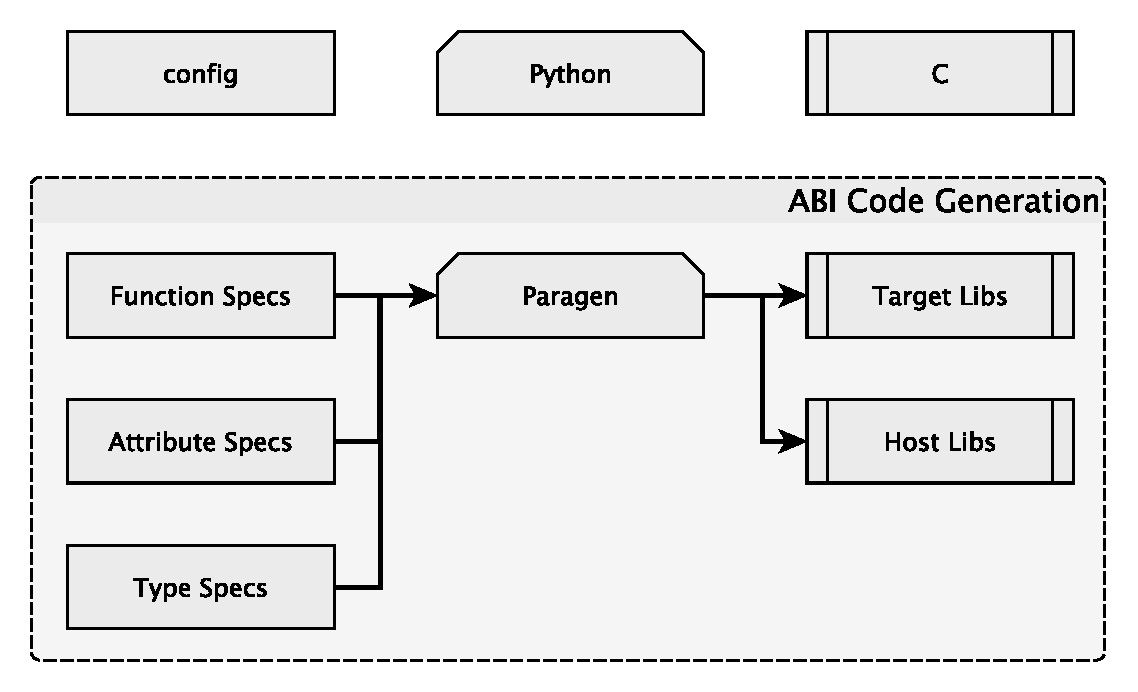
\includegraphics[width=\linewidth]{img/yedabigeneration.pdf}
  \caption[The framework generation process]{Visualization of the framework code generating process performed to compile the target- and host system libraries.}
  \label{fig:abigeneration}
\end{figure}

\subsection{Target System Libraries}
\label{sec:proposedsolutionandimplementation_targetsystemlibraries}
Compiled from \texttt{C} and \texttt{C++} sources output by the generation program, the target system libraries compose implementations of the EGL and OpenGL APIs.
Due to the tight coupling ibetween OpenGL and the platform windowing system, the solution must also accelerate the Khronos EGL API - the interface between OpenGL and the underlying platform windowing system.
As may be derived from the name, the target system libraries run on the simulation target system and replace any existing Khronos libraries.

Accordingly, the target system libraries implement the EGL and OpenGL~ES~$2.0$ APIs and lures whatever application it is being linked to that it is, in fact, the expected platform libraries.
Given that the target system libraries adheres to the OpenGL headers defined in the system, the application is na\"{\i}ve in terms of its paravirtualized status.
The interplay with the original OpenGL~ES headers also results in the solution adhering to the platform-dependent type definition, flags, and constants; as originally defined by Khronos.
However, instead of communicating with the platform windowing system (in terms of EGL) and the graphics device (in terms of OpenGL) - and instructing said device in accordance to the user; the target system libraries serialize the given command stream and forwards it to the simulation host.
However, the transmission of the command stream is not necessarily performed at once, or in the designated order, due to the formation of the OpenGL~ES~$2.0$ framework.
This complex of problems involve uncertainties of the proportion of argument data, as size is not necessarily given by the user or apperent at that time.
As such, certain serialization may have to be delayed until further information surrounding the argument dimensions have been relayed to the OpenGL library.
Furthermore, a subset of the OpenGL state need be maintained by the target system libraries.
These attributes are comprised by, inter alia, bound vertex- and index element buffers, in addition to properties of OpenGL vertex attributes.
Such states must be kept in the target system libraries due to the asynchronous nature of serialization of OpenGL invocations in the paravirtualized solution.

The serialization described in the above paragraph is thus formatted and encoded in accordance to a certain data format, which is kept as minimal as possible throughout execution.
This encoding includes packing variable length data types, such as $8$-bit characters, $16$-bit fields, or $64$-bit integer values, into fixed length structures, so that the host system may interpret these values independently of how corresponding types are defined on that unrelated platform.

%\footnote{It should be noted, however, that the solution assumes a little endian architecture and IEEE 754 standard for floating point representation. If the host system would not conform to these prerequisites, the solution would have to be complemented with additional support.}.

% Host System Libraries
\subsection{Host System Libraries}
\label{sec:proposedsolutionandimplementation_hostsystemlibraries}
In collaboration with the target system libraries, the host system libraries subsequently decodes and interprets the received byte stream.
Said decoding involves unpacking data from fixed length storage into variable-size types that OpenGL and EGL libraries expect.
Furthermore, and again similarly to the target system libraries, due to design inherent in the OpenGL~ES~$2.0$ framework, the host system libraries need maintain some data for state saving purposes.
Such data is buffered in the host system libraries until used (drawn) in a later, and separate, OpenGL invocation.
%\footnote{A possible optimization would be to cache said data, to avoid the need to transmit unmodified vertices multiple times, despite so being specified by the user.}.
When the requested OpenGL invocation has been performed, any return- or in-out values are returned to the target system using the Simics pipe.
As with the the target system libraries, the receiving end of an OpenGL method definitions in the host system libraries are likewise generated to a large degree.

% Windowing Systems
\subsection{Windowing Systems}
\label{sec:proposedsolutionandimplementation_windowingsystems}
Due to variations in the creation and maintenance of windows on different platforms (Fedora, Android, etc.), the window to which OpenGL renders is kept on the simulation host.
This incurs the dilemma of the target system libraries having to communicate with the fraudelent window to which OpenGL renders (in the simulation host) \textit{and} the native window (for example, reporting successful initialization).
After all, it would be problematic if the target OpenGL application would have to be modified in order to be paravirtualized.
Effectively, this means that it would be desirable to maintain the native functionality of the target system EGL library.
However, in order to swap the backbuffers to which OpenGL renders, one must use EGL.
In this way, the problem arises of a conflict between wanting to keep the functionality of the native EGL library, yet modify a small subset of it.
 
This issue is overcome by overriding symbols in the target libraries, which allows us to overload a function, serialize and forward the invocation to the host system, locate the next occurrence of the symbol in the symbol table (being the original native EGL function definition), and invoke the original function.
Accordingly, the target system EGL library does not replace the native target EGL library in its entirety, as with the OpenGL library, but rather extends it a bit.
This gives the effect of a successfully created window, not having returned any errors in the window creation and maintenance - yet having the application actually communicating with a different window.
As such, the target system libraries are effectively performing a man-in-the-middle attack on the target EGL library.

% Simics Pipe
\subsection{Simics Pipe}
\label{sec:proposedsolutionandimplementation_simicspipe}
The Simics pipe constitutes the target-to-host communications channel in Simics.
As such, it is responsible for transferring a serialized command stream to- and from the simulation host.
In order to do this, the pipe requires a way to exchange information with the outside world; a recurring issue in terms of virtual platforms.

There may be reasons as to why one would like to escape the simulation and resume execution in the real world.
Such a scenario would be a debugging breakpoint, to share data in-between target and host systems, or for any reason modify the simulation state.
There are a number of ways to communicate with the outside world (including the host machine) from within the simulation, such as by networking means or specially devised kernel drivers, but few are as instant as the - arguably - legitimately coined 'magic instruction'.

The magic instruction is a concept used to denote a \dvtcmdcodeinline{nop}-type instruction, meaning an instruction that would have no effect if run on the target architecture (such as \dvtcmdcodeinline{xchg ebx, ebx} on the x86), which, when executed on the simulated hardware in a virtual platform, invokes a callback-method in the simulation host~\dvtcmdcitebib[p.~32]{publications:leupers:2010}.
An advantage of this methodology is an often negligible invocation cost, as the context switch is often instant from the perspective of the target system~\dvtcmdcitebib[p.~131]{journals:rechistov:2013}.
Furthermore, being a greatly desirable attribute, magic instructions require no modification of the target system.
In effect, implementation of magic instructions requires replacing one- or more instructions in the target instruction set; thereby making the magic instruction platform-dependent.
However, the solution is often designed to only respond to magic instructions wherein a certain magic number, sometimes called a 'leaf number'~\dvtcmdcitebib[p.~131]{journals:rechistov:2013}, is present in an arbitrary processor register.

Due to the inherent performance demands brought on by serialization of real-time graphics invocations, magic instructions are a suitable candidate to exchange information between target host systems.
Magic instructions allow for fast, in the pretext of the simulation target - almost instant - escape from the simulation context, and may carry a limited amount of information with it from inside the simulation out into the real world.
The role of the Simics pipe is comprised of the allocation and maintenance of page locked target memory to accomodate the use of magic instructions; which the Simics pipe uses to relay the starting address of said memory space to the simulation host.

During a magic instruction, we may write an arbitrary 64-bit address to any register fit for purpose (the number and size of processor registers being the data-sharing bottleneck of the method).
Not being the first time magic instructions have been used for the purposes of hardware acceleration~\dvtcmdcitebib[p.~32]{publications:leupers:2010}, the Simics Pipe utilizes such methodology, namely the \dvtcmdcodeinline{CPUID} x86 instruction, to carry a lone memory address (the starting address of the serialized command stream) in one of the target system registers.
The execution of the injected instruction in a simulated processor invokes a callback method in the host side of the Simics Pipe; having effectively escaped the simulation and paused the simulation state.
Knowing the occurrence of a magic instruction with the corresponding leaf number, one may assume the existence of a target memory address in the simulated target CPU register, as agreed upon.
Note that, at this point, the retrieved address is in the format of a target system virtual address; the destination of which is unknown to the simulation host.
As such, this address need be translated in order to retrieve the package contents said memory address points to.

\begin{figure}
\centering
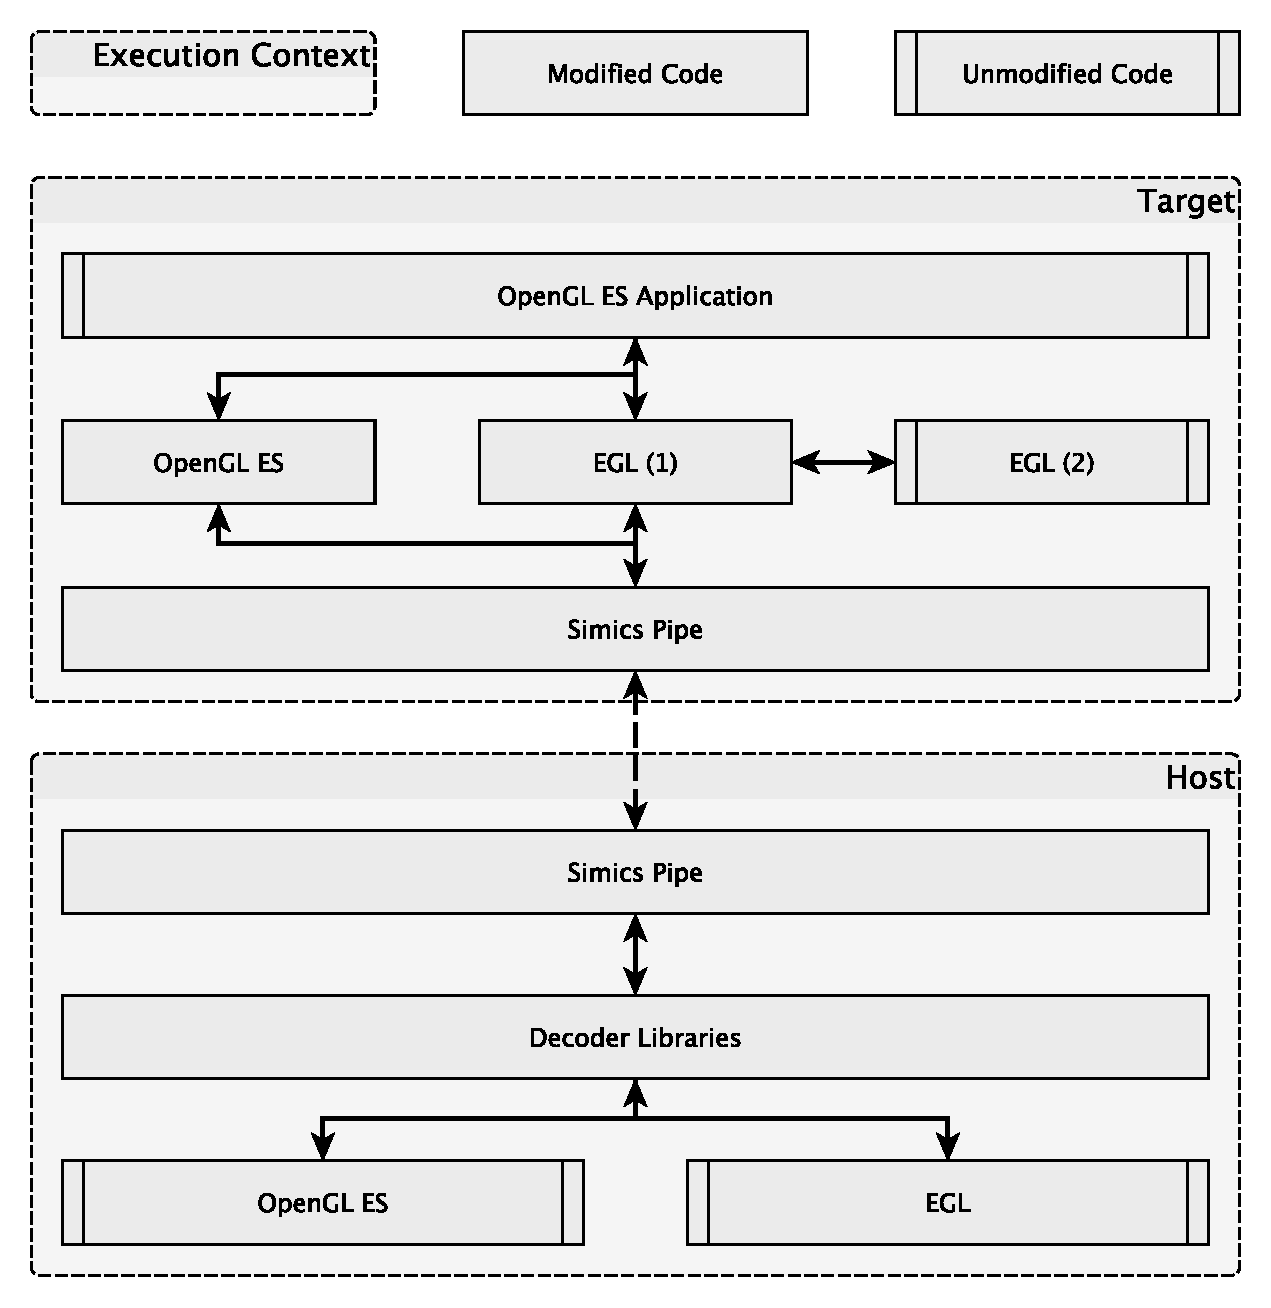
\includegraphics[width=\linewidth]{img/yedoverview.pdf}
\caption[Paravirtualization implementation overview]{Overview of the implementation accomodating paravirtualized graphics in Simics.}
\label{fig:overview}
\end{figure}

% Page Table Traversal
\subsection{Page Table Traversal}
\label{sec:proposedsolutionandimplementation_pagetabletraversal}
As outlined in section \ref{sec:proposedsolutionandimplementation_simicspipe}, target and host memory sharing is performed by the means of exposing a target virtual address to the simulation host.
Using Simics to access the MMU of the target system, one may translate a target virtual address to a (target) physical device address; to/from which we may access an arbitrary number of bytes in physical memory.
However, due to the complexity induced by circumventing the abstraction of virtual memory, there is no guarantee that the memory page to which the exposed physical address refers has not been swapped out of primary memory.
In order to solve this, we must 'lock' target system memory pages to prevent them from being swapped to disk.
This is the methodology used to ensure that the physical memory space, referred to by the virtual address sent to the simulation host, is still present in target primary memory when the simulation state is paused.
Other methods to achieve this include repeatedly 'polling' the corresponding memory pages in the target system.

Furthermore, and again induced by the unorthodox circumvention of the virtual memory paradigm, it is probable that the multiple memory pages making out particularly large serialized command streams, such as the transmission of vertex or texture data, are not consecutively aligned in physical memory, although guaranteed to be continuous blocks in terms of virtual memory.
As such, the physical addresses of memory pages must be continuously retrieved and translated on a per-page basis; effectively 'traversing' the virtual memory table (see figure \ref{fig:virtualmemory}).
This can be done in a trivial manner by simply iterating the original virtual address with the (target) page size.
In our case, $4096$ bytes.
Naturally, said process must be performed regardless of data being read or written to-/from the intended (physical) memory space.

\begin{figure}
\centering
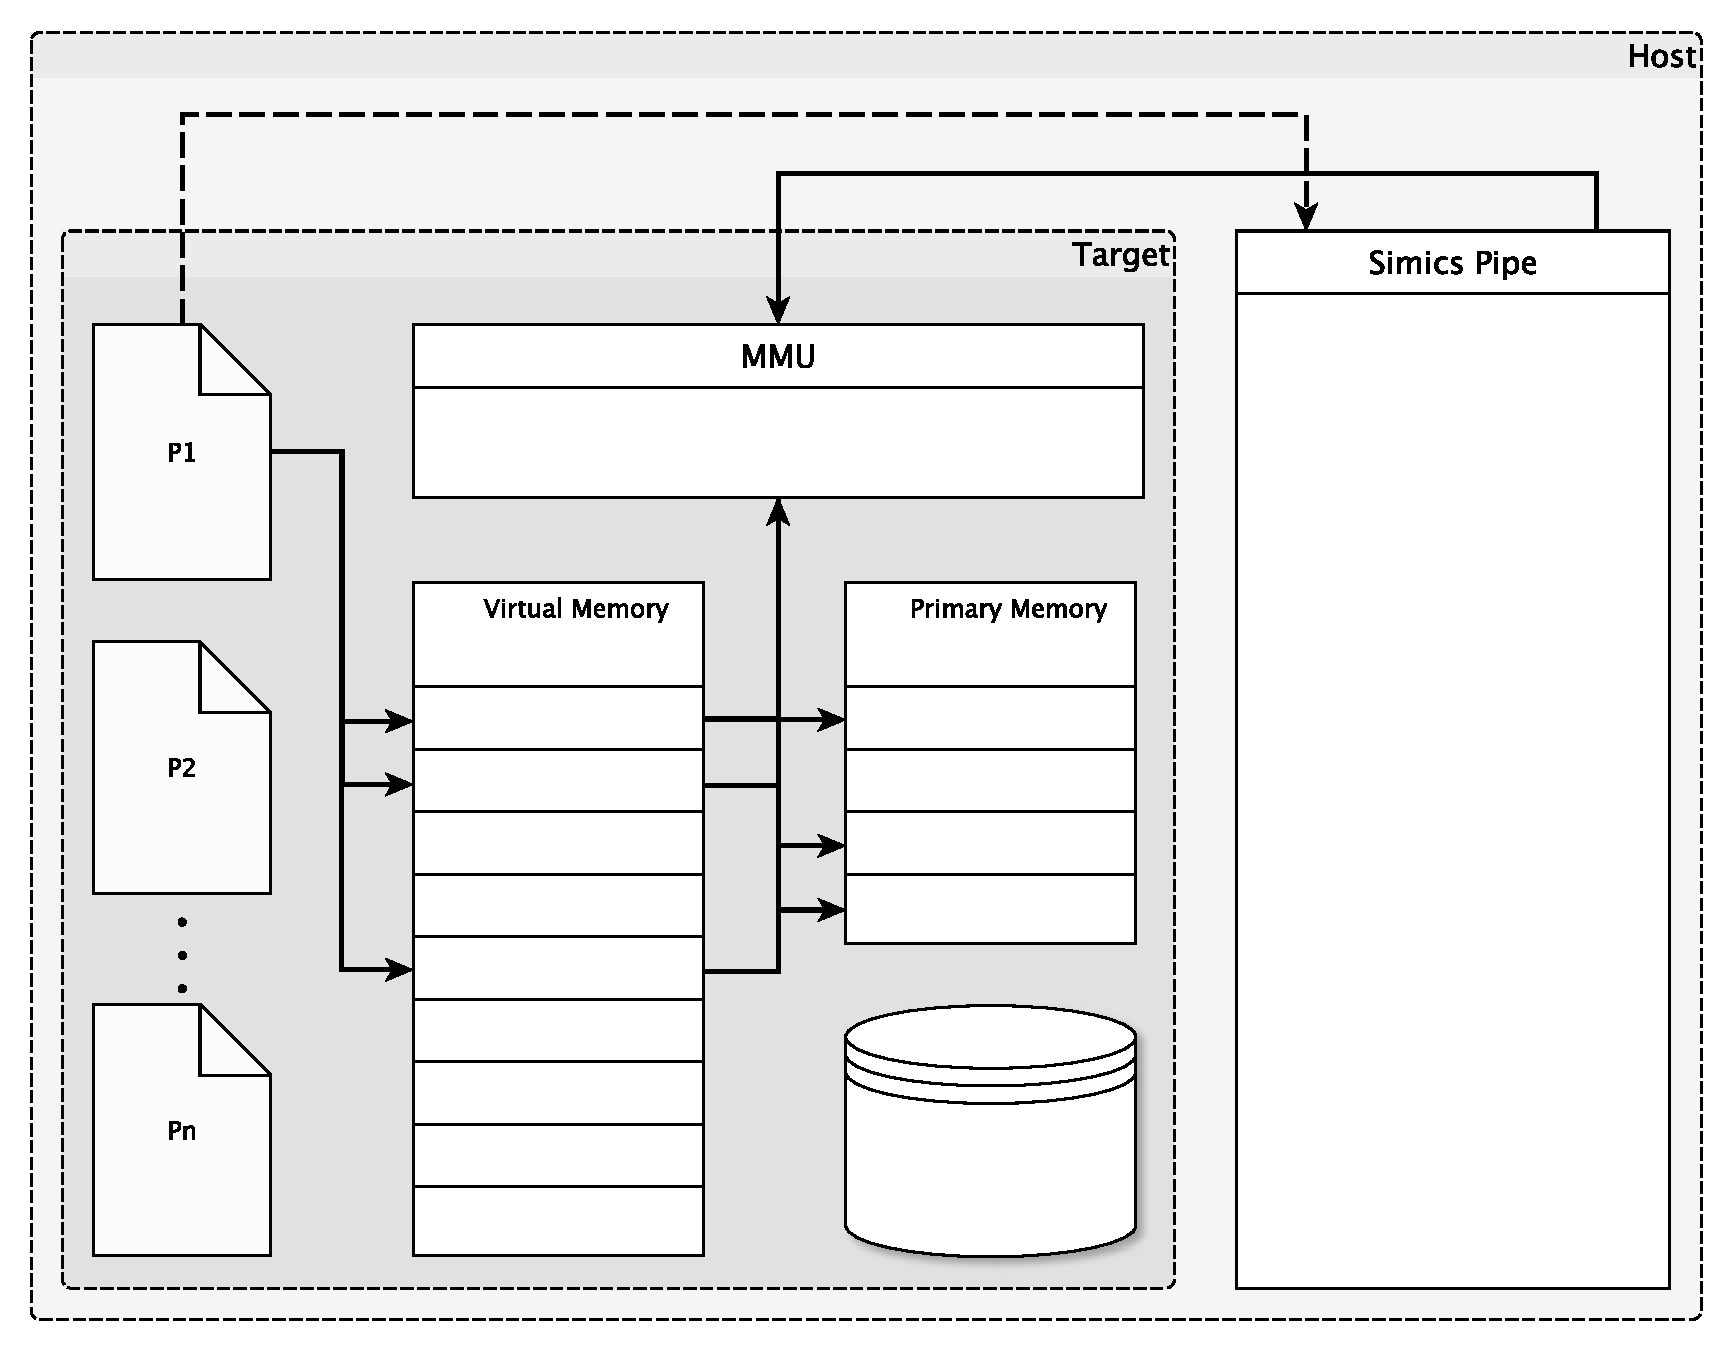
\includegraphics[width=\linewidth]{img/yedvirtualmemory.pdf}
\caption[Memory translation overview]{\hl{Memory translation overview. The OpenGL process hands a virtual memory address, pointing somewhere in the target system \textit{primary} memory, to the paravirtualized solution - which inquiries the target system MMU to retrieve designated bytestream directly from target physical memory.}}
\label{fig:virtualmemory}
\end{figure}

\subsection{Experimental Methodology}
\label{sec:experimentalmethodology}
The experiment is performed in software rasterized- and paravirtualized Simics platforms, respectively, in addition to reference runs on the host system.
Simics is configured to simulate an Intel\circledR\ Core \texttrademark\ i7; the same processor series to that of simulation host hardware.
During simulation, we utilize KVM to accelerate simulation by running target x86 instructions natively on host (x86) hardware.
The simulation systems are, like the host system, set up to run Fedora $19$ Linux and use the Mesa llvmpipe driver for OpenGL software rasterization.

The system upon which the experiment is performed is an x86-compatible Haswell Intel\circledR system running Fedora 19 Linux with the following specifications:
\todo{Add host system specs.}

% TODO: include in document or remove.
% QEMU SETUP
%% For QEMU reference tests, we profile the performance of the (QEMU) Android emulator to relate the devised solution to pre-existing technologies, in addition to execution on the hardware accelerated host platform as a reference case.
%% In order to accommodate for similar acceleration in QEMU, Android is configured to run on the Intel\circledR Android x86 system image (see \dvtcmdciteref{technicaldocs:intel:2013:x86}), circumventing the need to interpret ARM instructions~\dvtcmdciteref{web:stylianou:2010}.
%% Furthermore, the solution also utilize KVM in order to provide similar native execution on the host hardware\footnote{Had the solution been running on the Windows OS, the solution would have utilized Intel\circledR\ HAXM (see ~\dvtcmdciteref{technicaldocs:intel:2013:haxm}) to accommodate for said native execution~\dvtcmdciteref{web:hofemeier:2010}.}.
%% %Paravirtualized Android $4.4$\footnote{Android KitKat - API level $19$.} QEMU target system

% Benchmarks
\subsubsection{Benchmarks}
\label{sec:experimentalmethodology_benchmarks}
Throughout the course of the pilot study, no existing OpenGL~ES~$2.0$ benchmark (featuring cross-platform profiling support for \hl{Android} and X11 Linux) was deemed appropriate for for the purposes of this experiment.
As such, a pair of benchmarks have been devised on-site for the purposes of stress-testing the paravirtualized technology described in this document.
The benchmarks are intended to stress suspected bottlenecks in the implementation; a large number of relatively insignificant OpenGL~ES invocations and computationally intensive GPU workload.
These benchmarks are configured to run at roughly $16$~\milli\second , which would correspond to roughly $60$~frames per second, when hardware accelerated on the host system.
The benchmarks are devised in this way in order to reflect the expected load of a modern real-time interactive application.
As such, the purpose of developed benchmarks is to be representative of typical scenarios induced by modern graphics applications whilst utilizing a graphics framework such as OpenGL.
When run during the experiment, each benchmark instance measures the elapsed time of $1000$ frames which makes up the data subsequently analyzed.
Frame captures of the benchmarks are presented in figures \ref{fig:benchmarks_chess} and \ref{fig:benchmarks_julia}.

In order to detect anything but linear potential of scaling in software rasterized- and paravirtualized Simics platforms,  we run the benchmarks in three separate instances, respectively.
These benchmark versions differ in terms of input data; where said input is a changed variable that could potentially worsen benchmark performance (e.g., more vertex points).
The purpose of this is to detect any unexpected results in execution; and thus identify any performance complexity issues in software rasterized- and paravirtualized Simics platforms.
For consistency, each variation - of which there are two; resulting in three unique experiments per benchmark - have been produced to halve- and subsequently double the corresponding input data.
The described input data, for each benchmark, is presented in table \ref{tab:keyvals}.
Consequently, in table \ref{tab:keyvalsmagicinstructions}, the per-frame number of magic instructions induced by these input data variations are presented, differing only for the Chess benchmark.

% tab:keyvals
\begin{table}
  \centering
  \begin{tabular}{lllll}
    Benchmark & Input Data & Halved Input & Ref. Input & Double Input \\ \hline
    Chess & No. Tiles & $60\times60$ & $84\times84$ & $118\times118$ \\
    Julia & No. Iterations & $225$ & $450$ & $900$ \\
  \end{tabular}
  \caption[Input data variations]{Input data used for benchmark variations for each benchmark.}
  \label{tab:keyvals}
\end{table}

% tab:keyvalsmagicinstructions
\begin{table}
  \centering
  \begin{tabular}{lllll}
    Benchmark & \phantom{Input Data} & Halved Input & Ref. Input & Double Input \\ \hline
    Chess & \phantom{No. Tiles} & $32403$ & $63507$ & $125319$ \\
    Julia & \phantom{No. Iterations} & $16$ & $16$ & $16$ \\
  \end{tabular}
  \caption[Input data variation magic instruction count]{Number of magic instructions performed per-frame for each benchmark input data variation.}
  \label{tab:keyvalsmagicinstructions}
\end{table}

Note that for each tile rendered in the Chess benchmark, the solution will perform $9$ magic instructions; entailing a total of $32400$ ($9\times60\times60=32400$), $63504$ ($9\times84\times84=63504$), and $125316$ ($9\times118\times118=125316$) magic instructions, respectively, in addition to a minor number per-frame.

\begin{figure}
  \minipage{0.5\linewidth}
  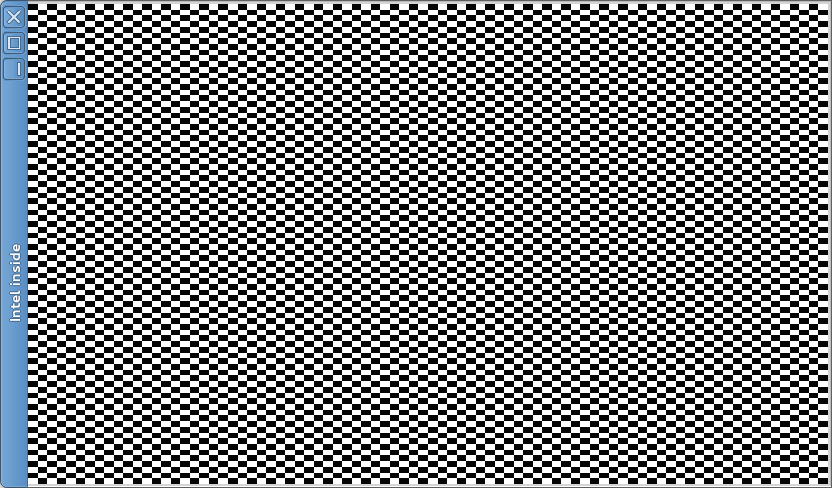
\includegraphics[width=\linewidth]{img/imgchess.png}
  \caption[Chess benchmark screen capture]{Chess.}
  \label{fig:benchmarks_chess}
  \endminipage\hfill
  \minipage{0.4\linewidth}
  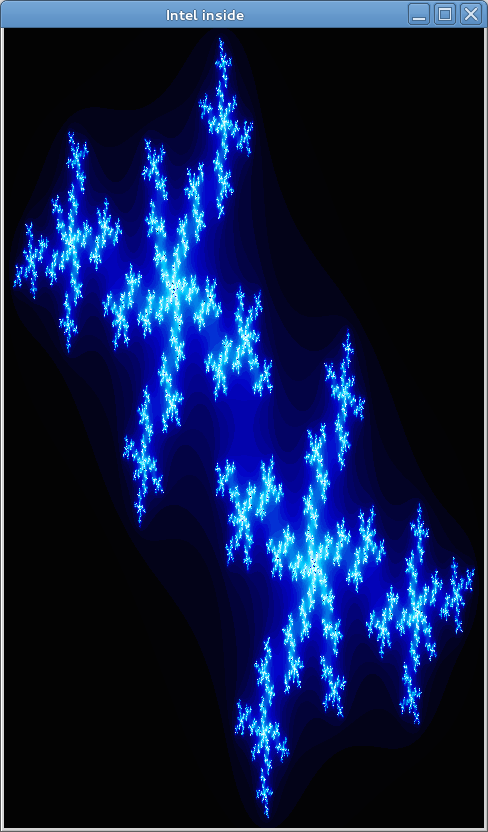
\includegraphics[width=\linewidth]{img/imgjulia.png}
  \caption[Julia benchmark screen capture]{Julia.}
  \label{fig:benchmarks_julia}
  \endminipage
\end{figure}

% Benchmark: Chess
\paragraph{Benchmark: Chess}
\label{par:experimentalmethodology_benchmarking_benchmarkchess}
\index{Chess benchmark}
The 'Chess' benchmark is developed for the purposes of stressing the latency in-between target - and host systems.
It is so named because of the chess-like tileset the graphics kernel produces.
The benchmark is designed to perform a multitude of OpenGL~ES~$2.0$ library invocations per frame; in which each invocation is relatively lightweight in execution and carry a small amount of data argument-wise.
In the Chess benchmark, this is achieved by rendering a grid of colored (black or white, in order to adhere to the chess paradigm) rectangles where each tile is represented by four two-dimensional vertices in screen-space, in addition to six indices outlining the rectangular shape.
Since the vertices are already transformed into screen-space, the graphics kernel need perform no additional transformation, adhering to the desired lightweight behavior of each kernel invocation.
Additionally, the tileset vertices and indices are pre-loaded into OpenGL vertex- and index element buffers, so that a lone buffer identifier may be carried over in-place of the heavier vertex set load.
Each tile is then individually drawn to the backbuffer, rendering the chess-like appearance of the benchmark.
Effectively, this means that, for each tile, the benchmark need only bind a vertex- and an index element buffer, set the corresponding tile color, and lastly invoke the rendering of said tile.

For each frame rendered, depending on the number of drawn tiles, the solution will perform a large number of magic instructions.
This induces a high utilization of the Simics Pipe, which is intended to stress magic instruction overhead (section \ref{sec:results_magicinstructionoverhead}).
The repeated invocation of lesser draw calls is representative of common usage of drawing a multitude of shapes with OpenGL, such as a user interface. Additionally, the number of tiles being computed is easily modifiable; rendering the benchmark scalable for the purposes of the experiment described in this document. As such, said benchmark is considered suitable for the purpose of representing a large number of graphics invocations using OpenGL~ES~$2.0$.

% Benchmark: Julia
\paragraph{Benchmark: Julia}
\label{par:experimentalmethodology_benchmarking_benchmarkjulia}
\index{Julia fractal benchmark}
The 'Julia' benchmark is developed for the purposes of stressing computational intensity in software-rasterized and paravirtualized platforms.
It is so named due to the kernel calculating the Julia fractal; the texturing and frame-wise seeding of which gives the benchmark it's distinct look.
The benchmark is designed to perform a lone computationally intensive graphics kernel invocation, which will stress the computational prowess of the profiled platform.
The case is selected for use as the computation of a fractal is trivially scalable in terms of complexity, by modifying the number of iterations the fractal algorithm performs, and is thus considered suitable for profiling of computationally intensive graphics kernels.

\subsection{Results}
\label{sec:results}
In this chapter, the results collected from having applied the described experiment methodology onto the devised solution are presented.
As such, the results gathered from execution on the host is presented in figure \ref{fig:histogramshost}, the results compiled from execution in the \hl{Android emulator presented in figure} \ref{fig:histogramsqemu}, and the results accumulated from software rasterized- and paravirtualized execution in Simics are presented in figures \ref{fig:histogramssimicsparachess} and \ref{fig:histogramssimicsparajulia}.

In this chapter, the results are compiled into histograms; visualizing elapsed time in milliseconds to sample density.
As such, the $Y$ axis showcase sample density; although the axis keys have been removed as they bear little relevance to the outcomes presented in this material.
The histograms each feature $100$ bins; into which a $1000$ samples, for each experiment performed, are rounded into.
For the purposes of good visualization methodology, values outside of the standard deviation\footnote{That is; values above that of the $mean + std$ and values under that of $mean - std$.} are not featured in the figures presented in this section.
In order to accommodate for the, however few, samples outside of said limits the figures are all complemented with key ratio tables (see tables \ref{tab:keyvalhost}, \ref{tab:keyvalqemu}, \ref{tab:keyvalsimics}, and \ref{tab:keyvalpara}).

% Benchmark Results
\subsubsection{Benchmark Results}
\label{sec:results_benchmarkresults}
Based on the reference profiling presented in figure \ref{fig:histogramshost}, we may conclude that the benchmarks, when hardware accelerated on the host system, perform with concentrated density; not being much scattered across the graph except a few irregular extremities in terms of maximum frame times (see table \ref{tab:keyvalhost}).
This is supported by the standard deviation presented in said table.
Furthermore, we may conclude that the Phong demo features two distinct peaks in density distribution - about $1$ ms in-between.
There may be cause to believe that this is caused, or partly caused, by frame-wise rotation of the teapot - rotation featured in the benchmark (see section \ref{sec:experimentalmethodology_benchmarks}) - inducing some fluctuation into its execution (see figure \ref{fig:histogramssimicsparaphong}).
However, this behavior is, strangely so, not apparent whilst paravirtualized in the QEMU derived Android emulator, although this may be a visual artifact due to the resolution of the graph (see figure \ref{fig:histogramsqemu}).
See section \ref{sec:threatstovalidity_benchmarkvariations} for an elaboration on divergence in the Phong benchmark.
Additionally, and in accordance to tables \ref{tab:keyvalhost} and \ref{tab:keyvalqemu}, one may observe relatively high recorded maximum frame times in relation to compiled maximum- and average values, yet featuring - in relation to divergent maximum, relatively low standard deviations.

The remainder of this chapter will present a benchmark-wise analysis of the data compiled from executing the experiment on the software rasterized- and paravirtualized Simics platforms; said platforms being the subject of this study.
For the sake of brevity, these analyses are segmented into paragraphs for each benchmark.
These paragraphs are presented below.

\begin{figure}
  \centering
  \input{gnuhistogramshost.tex}
  \caption[Benchmark results - hardware accelerated on the simulation host]{Histogram depicting benchmark elapsed frametimes in milliseconds and the density distribution of 1000 frames whilst hardware accelerated on the simulation host. The $Y$ axis thus depict sample density. Its axis keys have been removed as they bear no relevance to the outcomes presented in this document.}
  \label{fig:histogramshost}
\end{figure}

\begin{figure}
  \centering
  \input{gnuhistogramsqemu.tex}
  \caption[Benchmark results - paravirtualized in QEMU]{Histogram depicting benchmark elapsed frametimes in milliseconds and the density distribution of 1000 frames whilst paravirtualized in QEMU. The $Y$ axis thus depict sample density. Its axis keys have been removed as they bear no relevance to the outcomes presented in this document.}
  \label{fig:histogramsqemu}
\end{figure}

% tab:keyvalhost
\begin{table}
\centering
\begin{tabular}{|c|c|c|c|c|}
\hline
\multirow{2}{*}{Benchmark} & \multicolumn{4}{p{6cm}|}{\centering Elapsed time (milliseconds)} \\
\cline{2-5} & \multicolumn{1}{c|}{Min} & \multicolumn{1}{c|}{Max} & \multicolumn{1}{c|}{Std} & \multicolumn{1}{c|}{Avg} \\ \hline
Chess & \dvtcmdfirstline{hostchess84x84.dat.min} & \dvtcmdfirstline{hostchess84x84.dat.max} & \dvtcmdfirstline{hostchess84x84.dat.std} & \dvtcmdfirstline{hostchess84x84.dat.avg} \\ \hline
Julia & \dvtcmdfirstline{hostjulia450.dat.min} & \dvtcmdfirstline{hostjulia450.dat.max}	& \dvtcmdfirstline{hostjulia450.dat.std} & \dvtcmdfirstline{hostjulia450.dat.avg} \\ \hline
Phong & \dvtcmdfirstline{hostphong2048x2048.dat.min} & \dvtcmdfirstline{hostphong2048x2048.dat.max} & \dvtcmdfirstline{hostphong2048x2048.dat.std} & \dvtcmdfirstline{hostphong2048x2048.dat.avg} \\ \hline
\end{tabular}
\caption[Benchmark results - hardware accelerated on the simulation host]{Benchmarking results whilst hardware accelerated on the simulation host system.}
\label{tab:keyvalhost}
\end{table}

% tab:keyvalqemu
\begin{table}
\centering
\begin{tabular}{|c|c|c|c|c|}
\hline
\multirow{2}{*}{Benchmark} & \multicolumn{4}{p{6cm}|}{\centering Elapsed time (milliseconds)} \\
\cline{2-5} & \multicolumn{1}{c|}{Min} & \multicolumn{1}{c|}{Max} & \multicolumn{1}{c|}{Std} & \multicolumn{1}{c|}{Avg} \\ \hline
Chess & \dvtcmdfirstline{qemuchess84x84.dat.min} & \dvtcmdfirstline{qemuchess84x84.dat.max} & \dvtcmdfirstline{qemuchess84x84.dat.std} & \dvtcmdfirstline{qemuchess84x84.dat.avg} \\ \hline
Julia & \dvtcmdfirstline{qemujulia450.dat.min} & \dvtcmdfirstline{qemujulia450.dat.max}	& \dvtcmdfirstline{qemujulia450.dat.std} & \dvtcmdfirstline{qemujulia450.dat.avg} \\ \hline
Phong & \dvtcmdfirstline{qemuphong2048x2048.dat.min} & \dvtcmdfirstline{qemuphong2048x2048.dat.max} & \dvtcmdfirstline{qemuphong2048x2048.dat.std} & \dvtcmdfirstline{qemuphong2048x2048.dat.avg} \\ \hline
\end{tabular}
\caption[Benchmark results - paravirtualized in the Android emulator]{Benchmarking results whilst paravirtualized in the QEMU-derived Android emulator.}
\label{tab:keyvalqemu}
\end{table}

% tab:keyvalsimics
\begin{table*}
  \centering
  \providecommand{\chesskeyone}{$60\times60$ tiles}
  \providecommand{\chesskeytwo}{$84\times84$ tiles}
  \providecommand{\chesskeythree}{$118\times118$ tiles}

  \providecommand{\juliakeyone}{$225$ iterations}
  \providecommand{\juliakeytwo}{$450$ iterations}
  \providecommand{\juliakeythree}{$900$ iterations}

  \providecommand{\phongkeyone}{$1448\times1448$ texels}
  \providecommand{\phongkeytwo}{$2048\times2048$ texels}
  \providecommand{\phongkeythree}{$2896\times2896$ texels}

  \begin{tabular}{|c|c|c|c|c|c|}
    \hline
    \multirow{2}{*}{Benchmark} & \multirow{2}{*}{Key} & \multicolumn{4}{p{6cm}|}{\centering Elapsed time (milliseconds)} \\
    \cline{3-6} && \multicolumn{1}{c|}{Min} & \multicolumn{1}{c|}{Max} & \multicolumn{1}{c|}{Std} & \multicolumn{1}{c|}{Avg} \\ \hline
    \multirow{3}{*}{Chess} & \chesskeyone & \dvtcmdfirstline{simicschess60x60.dat.min} & \dvtcmdfirstline{simicschess60x60.dat.max}	& \dvtcmdfirstline{simicschess60x60.dat.std} & \dvtcmdfirstline{simicschess60x60.dat.avg} \\ %\cline{2-6}
    & \chesskeytwo & \dvtcmdfirstline{simicschess84x84.dat.min} & \dvtcmdfirstline{simicschess84x84.dat.max} & \dvtcmdfirstline{simicschess84x84.dat.std} & \dvtcmdfirstline{simicschess84x84.dat.avg} \\ %\cline{2-6}
    & \chesskeythree & \dvtcmdfirstline{simicschess118x118.dat.min} & \dvtcmdfirstline{simicschess118x118.dat.max} & \dvtcmdfirstline{simicschess118x118.dat.std} & \dvtcmdfirstline{simicschess118x118.dat.avg} \\ \hline
    \multirow{3}{*}{Julia} & \juliakeyone & \dvtcmdfirstline{simicsjulia225.dat.min} & \dvtcmdfirstline{simicsjulia225.dat.max} & \dvtcmdfirstline{simicsjulia225.dat.std} & \dvtcmdfirstline{simicsjulia225.dat.avg} \\ %\cline{2-6}
    & \juliakeytwo & \dvtcmdfirstline{simicsjulia450.dat.min} & \dvtcmdfirstline{simicsjulia450.dat.max} & \dvtcmdfirstline{simicsjulia450.dat.std} & \dvtcmdfirstline{simicsjulia450.dat.avg} \\ %\cline{2-6}
    & \juliakeythree & \dvtcmdfirstline{simicsjulia900.dat.min} & \dvtcmdfirstline{simicsjulia900.dat.max} & \dvtcmdfirstline{simicsjulia900.dat.std} & \dvtcmdfirstline{simicsjulia900.dat.avg} \\ \hline
    \multirow{3}{*}{Phong} & \phongkeyone & \dvtcmdfirstline{simicsphong1448x1448.dat.min} & \dvtcmdfirstline{simicsphong1448x1448.dat.max}	& \dvtcmdfirstline{simicsphong1448x1448.dat.std} & \dvtcmdfirstline{simicsphong1448x1448.dat.avg} \\ %\cline{2-6}
    & \phongkeytwo & \dvtcmdfirstline{simicsphong2048x2048.dat.min} & \dvtcmdfirstline{simicsphong2048x2048.dat.max} & \dvtcmdfirstline{simicsphong2048x2048.dat.std} & \dvtcmdfirstline{simicsphong2048x2048.dat.avg} \\ %\cline{2-6}
    & \phongkeythree & \dvtcmdfirstline{simicsphong2896x2896.dat.min} & \dvtcmdfirstline{simicsphong2896x2896.dat.max} & \dvtcmdfirstline{simicsphong2896x2896.dat.std} & \dvtcmdfirstline{simicsphong2896x2896.dat.avg} \\ \hline
  \end{tabular}
  \caption[Benchmark results - software rasterized in Simics]{Benchmarking results whilst software rasterized in the Simics full-system simulator.}
  \label{tab:keyvalsimics}
\end{table*}

% tab:keyalpara
\begin{table*}
  \centering
  \providecommand{\chesskeyone}{$60\times60$ tiles}
  \providecommand{\chesskeytwo}{$84\times84$ tiles}
  \providecommand{\chesskeythree}{$118\times118$ tiles}

  \providecommand{\juliakeyone}{$225$ iterations}
  \providecommand{\juliakeytwo}{$450$ iterations}
  \providecommand{\juliakeythree}{$900$ iterations}

  \providecommand{\phongkeyone}{$1448\times1448$ texels}
  \providecommand{\phongkeytwo}{$2048\times2048$ texels}
  \providecommand{\phongkeythree}{$2896\times2896$ texels}

  \begin{tabular}{|c|c|c|c|c|c|}
    \hline
    \multirow{2}{*}{Benchmark} & \multirow{2}{*}{Key} & \multicolumn{4}{p{6cm}|}{\centering Elapsed time (milliseconds)} \\
    \cline{3-6} && \multicolumn{1}{c|}{Min} & \multicolumn{1}{c|}{Max} & \multicolumn{1}{c|}{Std} & \multicolumn{1}{c|}{Avg} \\ \hline
    \multirow{3}{*}{Chess} & \chesskeyone & \dvtcmdfirstline{parachess60x60.dat.min} & \dvtcmdfirstline{parachess60x60.dat.max} & \dvtcmdfirstline{parachess60x60.dat.std} & \dvtcmdfirstline{parachess60x60.dat.avg} \\
    & \chesskeytwo & \dvtcmdfirstline{parachess84x84.dat.min} & \dvtcmdfirstline{parachess84x84.dat.max} & \dvtcmdfirstline{parachess84x84.dat.std} & \dvtcmdfirstline{parachess84x84.dat.avg} \\
    & \chesskeythree & \dvtcmdfirstline{parachess118x118.dat.min} & \dvtcmdfirstline{parachess118x118.dat.max} & \dvtcmdfirstline{parachess118x118.dat.std} & \dvtcmdfirstline{parachess118x118.dat.avg} \\ \hline
    \multirow{3}{*}{Julia} & \juliakeyone & \dvtcmdfirstline{parajulia225.dat.min} & \dvtcmdfirstline{parajulia225.dat.max}	& \dvtcmdfirstline{parajulia225.dat.std} & \dvtcmdfirstline{parajulia225.dat.avg} \\
    & \juliakeytwo & \dvtcmdfirstline{parajulia450.dat.min} & \dvtcmdfirstline{parajulia450.dat.max} & \dvtcmdfirstline{parajulia450.dat.std} & \dvtcmdfirstline{parajulia450.dat.avg} \\
    & \juliakeythree & \dvtcmdfirstline{parajulia900.dat.min} & \dvtcmdfirstline{parajulia900.dat.max} & \dvtcmdfirstline{parajulia900.dat.std} & \dvtcmdfirstline{parajulia900.dat.avg} \\ \hline
    \multirow{3}{*}{Phong} & \phongkeyone & \dvtcmdfirstline{paraphong1448x1448.dat.min} & \dvtcmdfirstline{paraphong1448x1448.dat.max} & \dvtcmdfirstline{paraphong1448x1448.dat.std} & \dvtcmdfirstline{paraphong1448x1448.dat.avg} \\
    & \phongkeytwo & \dvtcmdfirstline{paraphong2048x2048.dat.min} & \dvtcmdfirstline{paraphong2048x2048.dat.max} & \dvtcmdfirstline{paraphong2048x2048.dat.std} & \dvtcmdfirstline{paraphong2048x2048.dat.avg} \\
    & \phongkeythree & \dvtcmdfirstline{paraphong2896x2896.dat.min} & \dvtcmdfirstline{paraphong2896x2896.dat.max} & \dvtcmdfirstline{paraphong2896x2896.dat.std} & \dvtcmdfirstline{paraphong2896x2896.dat.avg} \\ \hline
  \end{tabular}
  \caption[Benchmark results - paravirtualized in Simics]{Benchmarking results whilst paravirtualized in the Simics full-system simulator.}
  \label{tab:keyvalpara}
\end{table*}

% Chess
\paragraph{Chess}
\label{par:results_chess}
From the data visualized in figure \ref{fig:histogramssimicsparachess}, we may observe that the Chess benchmark, when executed in the software rasterized Simics platform, has a relatively broad distribution of its sample density, yet the distribution often seems evenly distributed around a single point.
The right-hand side of the graph, although also showcasing the impaired performance of the corresponding (paravirtualized) platform, visualizes a decrease in the distribution of the sample density.
This is supported by the data presented in table \ref{tab:keyvalpara}.

Based on the data summarized in table \ref{tab:keyvalsimics} (whilst software rasterized in Simics ) and comparing said data to that of table \ref{tab:keyvalpara} (whilst paravirtualized in Simics ), we may observe that the software rasterized solution outperforms it's paravirtualized counterpart; not only in the base experiment, but in all of its input data variations.
The only redeeming attributes the paravirtualized solution brings to the table, as elaborated upon in the above paragraph, is a decrease in the standard deviation of the benchmark profiling.
When comparing these results to the uncompromised hardware accelerated counterpart on the host machine (see figure \ref{fig:histogramshost}), we may observe - albeit considerably less prominent - an adherence to the single-peak behavior in the distribution of the sample density.

The purpose of the Chess benchmark is to locate any bottlenecks related to the number of paravirtualized library invocations (see section \ref{sec:experimentalmethodology_benchmarks}), which was predicted during the pilot study performed for the sake of this experiment.
As such, as presented in section \ref{sec:results_magicinstructionoverhead} in combination with the shaping of the Chess benchmark as presented in section \ref{sec:experimentalmethodology_benchmarks}, there is cause to believe that the prediction of a probable bottleneck in the target - to host communication latency has been confirmed; arguably identifying the weakness of graphics paravirtualization in the Simics full-system simulator.
The conclusions that may be drawn from these further stresses analysis into what is the root cause for the target - to host latency for a multitude of paravirtualized method invocations.
Results related to this matter are presented in section \ref{sec:results_magicinstructionoverhead}. 
Indeed, if proceeding from the findings of section \ref{sec:results_magicinstructionoverhead}, magic instruction overhead accounts for the majority of the elapsed average when paravirtualized in Simics.

% fig:hostgramssimicsparachess
\begin{sidewaysfigure*}
  \centering
  \input{gnuhistogramssimicsparachess.tex}
  \caption[Benchmark results - paravirtualized in Simics, Chess]{Histograms depicting benchmark elapsed frametimes in milliseconds and the density distribution of 1000 frames for the Chess benchmark key figure variations whilst software rasterized- and paravirtualized in Simics. The $Y$ axis thus depict sample density. Its axis keys have been removed as they bear no relevance to the outcomes presented in this document.}
  \label{fig:histogramssimicsparachess}
\end{sidewaysfigure*}

% Julia
\paragraph{Julia}
\label{par:results_julia}
In figure \ref{fig:histogramssimicsparajulia}, we may observe double- to triple peak behavior in the distribution of the sample density; both in software rasterized- and paravirtualized platforms.
Albeit the hardware accelerated host profiling (see figure \ref{fig:histogramshost}) may, however minor, suggest such a pattern; it is by all means not significant.
We may observe similar behavior in the distribution of the sample density when profiling the same benchmark whilst paravirtualized in the QEMU -derived Android emulator (see figure \ref{fig:histogramsqemu}).
What causes this behavior is unclear, as frame-to-frame branching in the fractal algorithm is minor and ought not cause such a variance.

The Julia benchmark is incorporated into the experiment to establish how the paravirtualized solution performed under computational stress (see section \ref{sec:experimentalmethodology_benchmarks}).
Using this benchmark, a performance weakness in the software rasterized Simics platform has been identified, with frame times well above the two second mark (see table \ref{tab:keyvalsimics}); with the corresponding maximum frame time in the paravirtualized Simics platform measuring up to to a mere \dvtcmdfirstline{parajulia900.dat.max} ms.
With the Julia benchmark, as visualized in figure \ref{fig:histogramssimicsparajulia}, we have showcased radical performance improvements for computationally intensive graphics kernels and - in turn - identified the capabilities of graphics paravirtualization in the Simics full-system simulator.

% fig:histogramssimicsparajulia
\begin{sidewaysfigure*}
  \centering
  \input{gnuhistogramssimicsparajulia.tex}
  \caption[Benchmark results - paravirtualized in Simics, Julia]{Histograms depicting benchmark elapsed frametimes in milliseconds and the density distribution of 1000 frames for the Julia benchmark key figure variations whilst software rasterized- and paravirtualized in Simics. The $Y$ axis thus depict sample density. Its axis keys have been removed as they bear no relevance to the outcomes presented in this document.}
  \label{fig:histogramssimicsparajulia}
\end{sidewaysfigure*}

% Magic Instruction Overhead
\subsubsection{Magic Instruction Overhead}
\label{sec:results_magicinstructionoverhead}
In Simics, magic instructions incur a context switch cost when exiting the simulation and beginning execution in the real world.
This affects the performance by forcing the simulation to no longer be executed in native mode; inhibiting the simulatory performance improvements granted by hardware-assisted virtualization.
It also entail Simics no longer being able to utilize just-in-time compilation to speed up execution; having to rely on regular code interpretation.
As such, in great numbers, magic instructions may potentially affect performance.

Considering the effect that this overhead may have on benchmarks such as Chess, we have performed additional experiments to establish the overhead costs.
The findings of the experiment are presented in \ref{tab:magicinstructionsforall}

\begin{table}
  \centering
  \begin{tabular}{llll}
    Min & Max & Std & Avg \\ \hline
    \dvtcmdfirstline{magicinstrprofileall.dat.min} & \dvtcmdfirstline{magicinstrprofileall.dat.max} & \dvtcmdfirstline{magicinstrprofileall.dat.std} & \dvtcmdfirstline{magicinstrprofileall.dat.avg} \\
  \end{tabular}
  \caption[Magic instruction profiling tabular, per-batch]{Profiling results for batched magic instructions. Presented in milliseconds and modified in accordance to the profiling overhead established in section \ref{sec:threatstovalidity_platformprofiling}.}
  \label{tab:magicinstructionsforall}
\end{table}

From these findings, we may conclude that the execution of $1000$ magic instructions is expected to induce an average overhead of roughly \dvtcmdfirstline{magicinstrprofileall.dat.avg} ms, accounting for profiling errors as presented in section \ref{sec:threatstovalidity_platformprofiling}.
Thus, the established overhead cost for $1000$ magic instructions is summarized in table \ref{tab:magicinstructionsforall}.

% Platform Comparison
\subsubsection{Platform Comparison}
\label{sec:analysisexperiment_platformcomparison}
\todo{This sections should be moved or removed depending on whether or not we bring up QEMU.}
In the sections above, results have been presented indicating performance gains, and potential for gains, in Simics platforms by the means of accelerating graphics using paravirtualization.
However, in accordance to figure \ref{fig:histogramsqemu} and table \ref{tab:keyvalqemu}, the platform on which the these results have been produced also utilizing paravirtualized methodology, there is much potential for improvement.
The benchmarks, when executed in the paravirtualized Android emulator, exhibit better performance in each test performed for the purposes of this paper; most notably outperforming the software rasterized Simics platform for the Chess benchmark.
The Chess benchmark, incurring such an overhead when paravirtualized in Simics (see paragraph \dvtcmdrefname{par:results_chess}) due to overhead induced by magic instructions (see section \ref{sec:results_magicinstructionoverhead}), performs but roughly two times worse than its hardware accelerated counterpart at \dvtcmdfirstline{qemuchess84x84.dat.avg} milliseconds average (see tables \ref{tab:keyvalqemu} and \ref{tab:keyvalhost}).
These results indicate potential for improvement in the target -to-host communications in Simics.
In fact, considering the large similarities in the paravirtualized methodology for graphics acceleration these two platforms share, the reference performance of the QEMU -derived Android emulator may be considered a goal for a potential productification of paravirtualized graphics in the Simics full-system simulator.

These comparisons suggest that the recorded performance for the benchmarks, devised for the purpose of this study, is not necessarily representative for paravirtualized graphics in general.
Furthermore, the comparison to the QEMU -derived Android emulator indicates that the shaping of the magic instruction -utilizing Simics Pipe - as established being the bottleneck during execution of the paravirtualized Chess benchmark (see section \ref{sec:results_magicinstructionoverhead}) - may have potential of improvement of approximately one order of magnitude (see tables \ref{tab:keyvalqemu} and \ref{tab:keyvalpara}).
